\hspace{24pt}
In this chapter, we review the related work in recent years. In section 2.1, we introduce the Burrows-Wheeler Aligner (BWA), a well-known alignment tool. In section 2.2, we introduce our previous research EAGLE, a method for evaluating the degree to which sequencing data supports a given candidate genome variant. In section 2.3, we explain what is reference bias and related solutions.
\section{Burrows-Wheeler Aligner}
Burrows-Wheeler Aligner (BWA) \cite{li2009fast} is a tool to align the sequences on selected large reference genomes such as human. It consists of three algorithms: BWA-backtrack, BWA-SW \cite{li2010fast} and BWA-MEM\cite{li2013aligning}. Among which BWA-MEM is the latest and generally recommended for high-quality queries as it is faster and more accuracy, basically replacing the first two algorithm.

Based on our read data and some previous studies, we believe that BWA-MEM will show better performance [HKL15], and its algorithm is robust to sequencing errors and applicable to a wide range of sequence lengths, so we decided to use BWA-MEM as our main algorithm for finding reads

BWA-MEM first needs to build the FM-index \cite{ferragina2005indexing} for the reference genome with the 'index' command.  The FM-index compressed substring index in based on the Burrows-Wheeler Transform (BWT) \cite{burrows1994block} and suffix array, generating a fast and efficient index for querying.

Then in the core alignment algorithm, BWA-MEM uses the seed-and-extend paradigm, and the process can be roughly divided into four steps. First step is seed, seed is found through super maximal exact matches (SMEM). Seconded step is re-seeding, in order to reduce the misalignment caused by missing seeds. Third step is chaining and filtering, chaining the seeds those are collinear and closed each other as a chain, and filter overlapped or short chain. Forth step seed extension, extending the seed in the chain to achieve the final exact match region.
\section{EAGLE: Explicit Alternative Genome Likelihood Evaluator}
EAGLE \cite{kuo2018eagle} is our previous research, based on a generative probabilistic model, variant calling evaluator, EAGLE main function is given individual sequencing data (exome or whole genome sequencing) and a list of candidate variants, and returns a likelihood score of each candidate variants.
The concept of EAGLE is that in the process of executing variant calling, there will be many uncertain factors, such as the error rate of alignment, low coverage sequencing and error rate of base-calling, etc., and these will affect downstream analysis. And EAGLE handles these possible errors and uncertainties through generative probabilistic model  (Figure~\ref{f2-1}).

\begin{figure}[H]
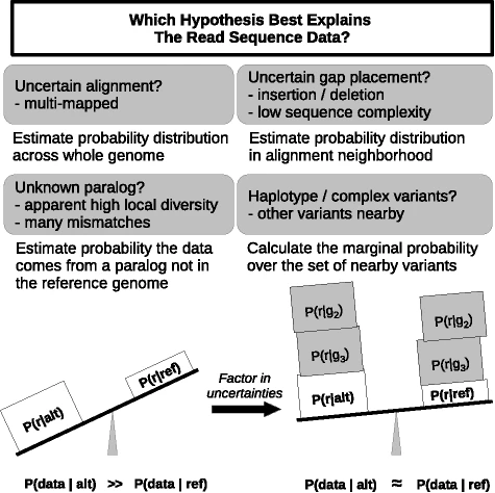
\includegraphics[width=0.6\columnwidth]{body/image/2-1.png}
\caption[EAGLE model]{EAGLE a use generative probabilistic model to handle uncertainty.}
\label{f2-1}
\end{figure}

Overall, the more uncertain the data the more uncertain the explanation.  Thus, in principal the likelihood computed by EAGLE can be used rank the reliability of putative variants.

\subsection{EAGLE computation flow}
At a technical level, EAGLE walks through two data files while scanning the genome.  The first file is a so-called BAM file, holding the information of reads mapped to one or more positions in the genome.  The second file is a so-called VCF file holding candidate genome variants.  Conveniently both of these file formats are sorted by genome position.  Our modified version of EAGLE maintains this structure and flow, but allows consideration of some relevant reads not present in the pileup.


\section{Reference Bias}
Sequencing data analysis often begins with aligning reads to a reference genome, but this sequence only contains the reference allele at polymorphic sites~\cite{martiniano2020removing}, which leads to reference bias (Figure \ref{f2-2}).  Reads that contain alternate alleles tend to misalignment or incorrect alignments \cite{chen2021reference}, so at heterozygous site, the reads containing the reference allele usually constitute the majority of the mapped reads.  These problems can cause false negative or false positive variant calls~\cite{gunther2019presence}

\begin{figure}[H]
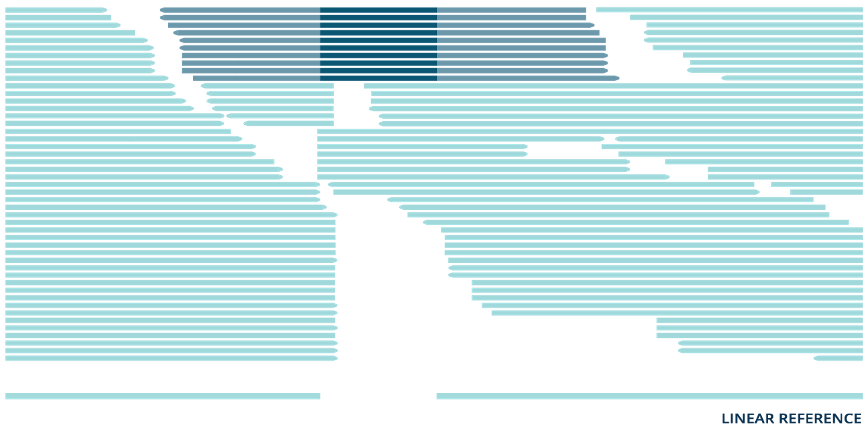
\includegraphics[width=1\columnwidth]{body/image/2-2.png}\vspace*{-1em}
\caption[Reference bias]{Reference bias. Only a small portion of the read containing inserts (dark blue) are mapped to the correct positions during the alignment to the reference genome.}
\label{f2-2}
\end{figure}
 

There have some studies discuss how to mitigate reference bias, such as genome graph aligners \cite{garrison2018variation,li2020design}, or using high-coverage NGS data, to improve the reference genome so that it includes the genomic diversity of the entire population.
In this paper, we modify the reference sequence to include alternate alleles, and try to find some matching reads to support this hypothetical sequence, then add these reads to the calculation of EAGLE to discuss the impact of this method on reducing reference bias and improve the accuracy of assessing variation.
